\documentclass[11pt]{report} % use larger type; default would be 10pt

\usepackage{mysty}
%%% The "real" document content comes below...
\newcommand{\horrule}[1]{\rule{\linewidth}{#1}} % Create horizontal rule command with 1 argument of height

\title{	
\normalfont \normalsize 
\textsc{International Institute of Information Technology, Bangalore} \\ [25pt] % Your university, school and/or department name(s)
\horrule{0.5pt} \\[0.4cm] % Thin top horizontal rule
\huge Analytics On A Subset Of The 2011 SSLC Data Set \\ Report \\ % The assignment title
\horrule{2pt} \\[0.5cm] % Thick bottom horizontal rule
}
%\title{Smart Water Networks \\ Project Report}
\author{Abhijith Madhav \and Saumya Tayal \and Nikita Shah}
%\date{} % Activate to display a given date or no date (if empty),
         % otherwise the current date is printed 

\begin{document}
\maketitle

\tableofcontents
\chapter{Data Preparation And Characterization}
\section{Data Preparation}
Prior preparation of data using a spreadsheet software
\begin{enumerate}
\item Have removed the '*'s in all of the marks column. 
\item Absentees have been given 0 marks in the respective subjects replacing the 888 marker.
\item Correcting totalling errors for about 21 records.
\item Added 'class' fields for each of the marks by using the following discretization. All marks attributes were scaled to 100.
\begin{itemize}
\item $< 35$ : FAIL
\item $< 50$ : PASS
\item $< 60$ : 2nd class
\item $< 85$ : 1st class
\item $> 84$ : Distinction
\end{itemize}
\item 
\end{enumerate}


Note : The following columns have the said number of rows with NA data. 
Shouldn't really matter as they are not being used in any of the experiments
\begin{itemize}

\item DOB = 1
\item NRC{\_}MOTHER{\_}NAME = 42
\item NRC{\_}FATHER{\_}NAME = 32
\item L1{\_}RESULT = 2
\item L2{\_}RESULT = 32
\item L3{\_}RESULT = 38

\end{itemize}
\section{Data Set Characterization}

\section{Code}
\texttt{https://github.com/AbhijithMadhav/SSLC-Data-Analysis}
\chapter{Discretization + Classification}
\label{chap:experiment1}

\section*{Objective}
To build a classification model for predicting the class of a student based on his course marks.

\section*{Procedure}
\begin{itemize}
\item Marks of all languages and subjects have already been discretized as in ~/ref{}
\item Built a classification model using a decision tree algorithm with L1{\_}CLASS, L2{\_}CLASS, L3{\_}CLASS, S1{\_}CLASS, S2{\_}CLASS, S3{\_}CLASS as predictors.
\begin{itemize}
\item Proportion of sizes of the training and test data sets were respectively 2/3 and 1/3.
\item Data records themselves were put into both the above data sets using random sampling.
\end{itemize}
\end{itemize}

\section*{Observations}
\begin{itemize}
\item Tabulation of the count of the predicted versus actual values for the test data set
\begin{lstlisting}
{
      pred
true      1    2 D    FAIL PASS
  1    2717  299   50    1    9
  2     613  920    0   23  350
  D     212    1  274    0    0
  FAIL    9   49    0 1894  558
  PASS   58  458    0  424 2081
}
\end{lstlisting}
\item Misclassification error
\begin{lstlisting}
0.2830909
\end{lstlisting}
\item Decision tree generated
\begin{figure}[h!]
  \caption{Decision Tree}
  \centering
    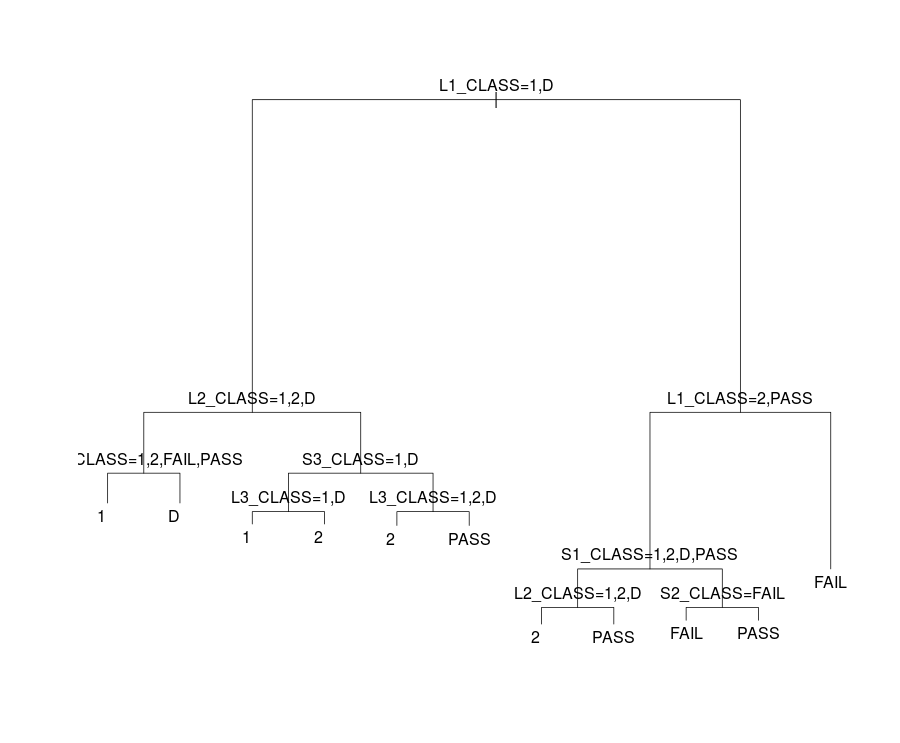
\includegraphics[scale=0.4]{img/rpart_nrc_class.png}
\end{figure}
\end{itemize}

\section*{Conclusions}
TODO
\chapter{Regression + Classification}

\section*{Objective}
Classification models using a lot of predictors give a model which might be complex. The objective thus is to try to use a simple linear regression model to determine the least number of attributes which affect the class to be predicted and then construct classification models.
\\
\\
Here the marks of the students are used to predict the NRC{\_}CLASS variable using a classification model.

\section*{Procedure}
\begin{itemize}
\item Marks of all languages and subjects have already been discretized as in ~/ref{chap:experiment1}.
\item Typically a linear regression model with more number of predictors gives a better fitted model. Thus for every count of the number of courses, from 1 to 5(not including all the courses), the best combination of predictors are chosen.
\begin{itemize}
\item For a number $n$,the best combination of predictors are found building regression models for all possible combination of attributes and the standard deviation of their residuals.
\end{itemize}
\item From each of these best combination of predictors a classification model is built.
\begin{itemize}
\item The classification model chosen is KNN as the predictors are numeric attributes. $k$ was chosen to be 10 after manual inspection with several values.
\end{itemize}
\item The accuracy of each of these classification models is compared to find out the best classification model.
\end{itemize}

\section*{Observations}
\begin{itemize}
\item Best predictors obtained
\begin{lstlisting}
> best_models
[[1]] # For n = 1
lm(formula = TOTAL_MARKS ~ S2_MARKS)

[[2]] # For n = 2
lm(formula = TOTAL_MARKS ~ L1_MARKS + L2_MARKS)

[[3]] # For n = 3
lm(formula = TOTAL_MARKS ~ L1_MARKS + L2_MARKS + S3_MARKS)

[[4]] # For n = 4
lm(formula = TOTAL_MARKS ~ L1_MARKS + L2_MARKS + S1_MARKS + S3_MARKS)

[[5]] # For n = 5
lm(formula = TOTAL_MARKS ~ L1_MARKS + L2_MARKS + L3_MARKS + S1_MARKS 
                           + S3_MARKS)
\end{lstlisting}
\item Comparision of misclassification errors for different number of predictors(Best combination)
\begin{figure}[h!]
  %\caption{Decision Tree}
  \centering
    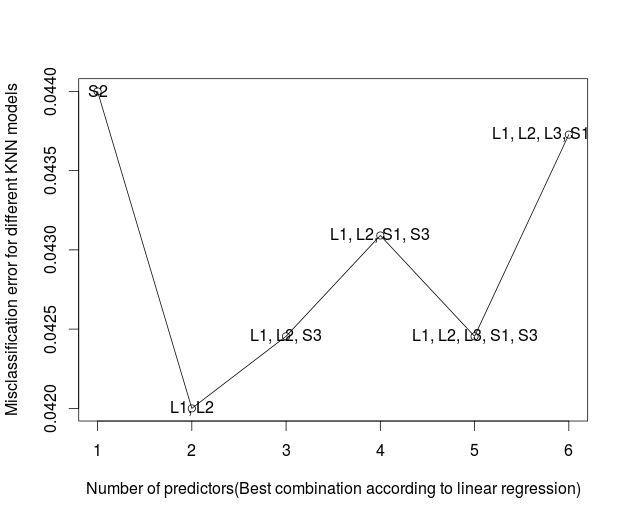
\includegraphics[scale=0.5]{img/error_knn.png}
\end{figure}
\end{itemize}

\section*{Conclusions}
\begin{itemize}
\item Marks of the first two languages(Typically Kannada and English) are the most accurate predictors of the NRC{\_}CLASS of a student.
\end{itemize}

\chapter{Clustering + Association Rules}
\label{chap:experiment3}
\section*{Objective}
Cluster characterization is most difficult part of clustering. Descriptive statistics are the standard way doing it. The objective here is to see if association rules will (hopefully) give a more intuitive explanation.

\section*{Procedure}
\begin{itemize}
\item Create a clustering of the students data set using the marks attributes.
\item KMeans is used and k is determined by using an elbow plot. The elbow plot was reasonably sharp at 4.
\item An extra column is added to the student dataset which contains the id of the cluster to which a particular record belongs to.
\item Association rules are generated by forcing the cluster id to be the antecedent to get the characterization of each cluster.
\end{itemize}

\section*{Observations}
\begin{itemize}
\item Elbow plot obtained

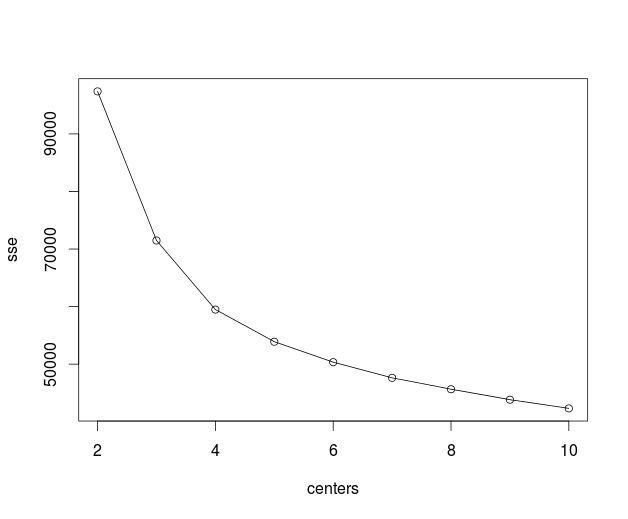
\includegraphics[scale=0.5]{img/kmeans_elbow.png}


\item Distribution around NRC{\_}CLASS
\begin{lstlisting}
       1    2 D    FAIL PASS
  1    1   57    0 2878 8780
  2 4554    0 1439    1    0
  3    0    0    0 4950    5
  4 4386 5669    1   32  249
\end{lstlisting}

\item Characterization using mean marks

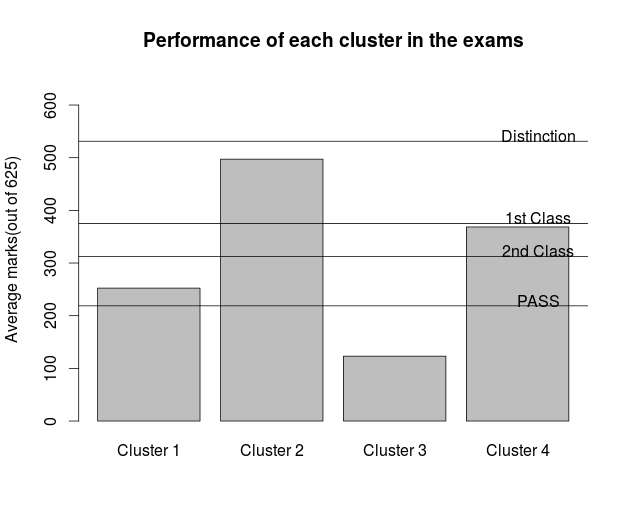
\includegraphics[scale=0.5]{img/barplot_mean_marks.png}


\item Visualization after reducing dimension to two using SVD

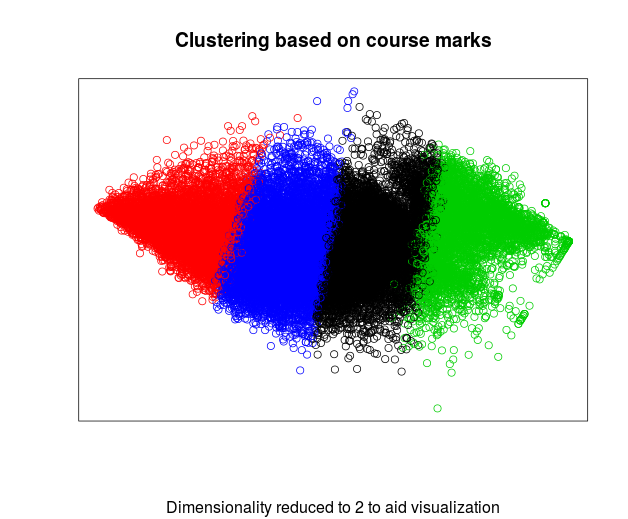
\includegraphics[scale=.5]{img/clusters_marks.png}




\item Association rules for each cluster
\begin{lstlisting}
> inspect(sort(cluster.rules))
   lhs               rhs                          support confidence     lift
1  {CLUSTER_ID=1} => {NRC_PHYSICAL_CONDITION=N} 0.3540695  0.9973540 1.0003245
2  {CLUSTER_ID=1} => {CANDIDATE_TYPE=RF}        0.3011333  0.8482417 0.9576707
3  {CLUSTER_ID=1} => {NRC_MEDIUM=K}             0.2771953  0.7808126 1.1236864
4  {CLUSTER_ID=1} => {NRC_CLASS=PASS}           0.2660445  0.7494025 2.7376336

5  {CLUSTER_ID=2} => {CANDIDATE_TYPE=RF}        0.1815042  0.9993327 1.128253
6  {CLUSTER_ID=2} => {NRC_PHYSICAL_CONDITION=N} 0.1813526  0.9984985 1.001472
7  {CLUSTER_ID=2} => {NRC_CASTE_CODE=4}         0.1536877  0.8461795 1.196368
8  {CLUSTER_ID=2} => {NRC_CLASS=1}              0.1379916  0.7597598 2.804339

9  {CLUSTER_ID=3} => {NRC_CLASS=FAIL}           0.1499909  0.9989909 4.1939573
10 {CLUSTER_ID=3} => {NRC_PHYSICAL_CONDITION=N} 0.1489607  0.9921292 0.9950841
11 {CLUSTER_ID=3} => {S2_CLASS=FAIL}            0.1335374  0.8894046 3.4110554
12 {CLUSTER_ID=3} => {S1_CLASS=FAIL}            0.1203866  0.8018163 3.9028825
13 {CLUSTER_ID=3} => {NRC_MEDIUM=K}             0.1198715  0.7983855 1.1489760
14 {CLUSTER_ID=3} => {L1_CLASS=FAIL}            0.1105994  0.7366297 4.2330232

15 {CLUSTER_ID=4} => {NRC_PHYSICAL_CONDITION=N} 0.3126477  0.9981619 1.001135
16 {CLUSTER_ID=4} => {CANDIDATE_TYPE=RF}        0.3112842  0.9938086 1.122017
17 {CLUSTER_ID=4} => {NRC_CASTE_CODE=4}         0.2308345  0.7369643 1.041954
18 {CLUSTER_ID=4} => {NRC_MEDIUM=K}             0.2207139  0.7046532 1.014084
\end{lstlisting}

\end{itemize}

\section*{Conclusions}
\begin{itemize}
\item Generating association rules on clusters is a satisfactory categorization technique. 
\item The lift is sometimes close to 1 which suggests independence. But this does not matter as the rules are not being interpreted as correlations between the lhs and rhs. The rhs just gives the categorization of the cluster. Lift close to one suggests the same categorization for other clusters.
\item The low support is also not a matter of concern as it is reflective of the measure w.r.t the whole dataset and not to the particular cluster.
\item Categorization : The categorization is as shown in the observations. The physical condition of students across clusters being normal is result of the lopsided distribution.
\end{itemize}

\chapter{Cross Cluster Analysis}

\section*{Objective}
To compare the cluster characteristics of a subset of the dataset with that of the whole dataset

\section*{Procedure}
\begin{itemize}
\item Partition the student dataset on a particular basis
\begin{itemize}
\item GENDER{\_}CODE
\item URBAN{\_}RURAL
\end{itemize}
\item Cluster the while dataset and the partitioned dataset separately and categorize the clusters
\begin{itemize}
\item Clustering and categorization is done as specified in ~ref{chap:experiment3}
\end{itemize}
\item Compare the categorization of clusters created out of each partitioned dataset with that of the clusters constructed using the whole dataset.
\end{itemize}

\section*{Observations}
\begin{itemize}
\item Partitioning based on GENDER{\_}CODE

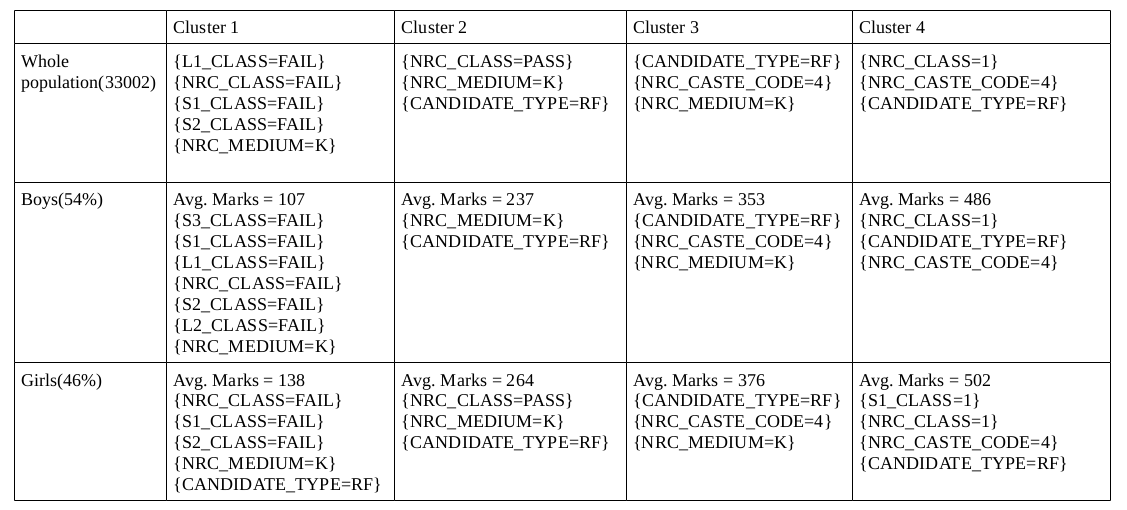
\includegraphics[scale=0.4]{img/boys_girls.png}

\item Partitioning based on URBAN{\_}RURAL

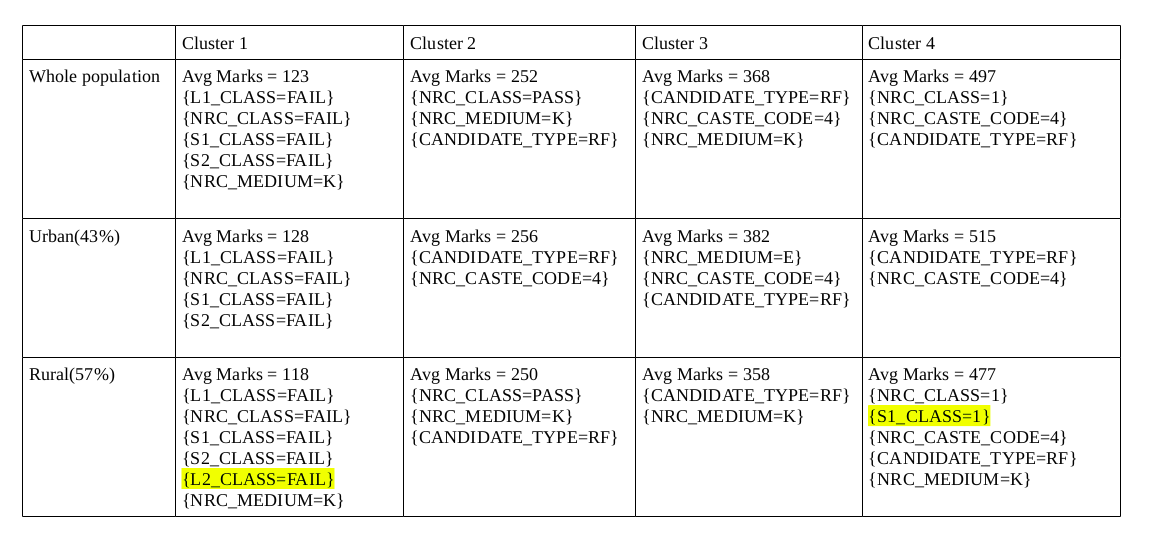
\includegraphics[scale=0.4]{img/urban_rural.png}

\end{itemize}


\section*{Conclusions}
\begin{itemize}
\item Partitioning based on URBAN{\_}RURAL

\begin{itemize}

\item Cluster 1 - Candidates who fail
\begin{itemize}
\item Urban - Their medium is not necessarily Kannada
\item Rural - They also fail in L2
\end{itemize}

\item Cluster 2 - Candidates who just pass
\begin{itemize}
\item Urban - Medium is not necessarily kannada and students belong to the general category.
\item Rural - Repeaters do not just pass. They either secure higher grades or fail(more likely).
\end{itemize}


\item Cluster 3 - Just missing First Class
\begin{itemize}
\item Urban - Medium is english.
\item Rural – Medium is kannada. Are not necessarily general category.
\end{itemize}



\item Cluster 3 - Just missing distinction
\begin{itemize}
\item Urban - There are a significant number of students who have gotten distinction.
\item Rural - Medium is kannada and have scored atleast 60 in mathematics.
\end{itemize}

\end{itemize}








\item Partitioning based on GENDER{\_}CODE

\begin{itemize}

\item Cluster 1 - Candidates who fail
\begin{itemize}
\item Boys - Fail in all subjects except L3, which is typically Hindi.
\item Girls - Do not fall in L1(Mostly Kannada). Most are regular freshers.
\end{itemize}

\item The other clusters have the same characteristics.

\end{itemize}


\end{itemize}

\end{document}

%--------------------------------------------------------------------------------------


